\customtitlepage{Through the PRISm: Importance-Aware Scene Graphs for Image Retrieval}{Zhen Wang, Zengrong Lin, Kun Huang, Cong Bai}

\section{Through the PRISm: Importance-Aware Scene Graphs for Image Retrieval}

\subsection{Abstract}
\begin{frame}{Abstract}
    \begin{block}{Challenge}
        In \texttt{Event Retrieval} or \texttt{Frame Retrieval} lies at the core of CV tasks. Most of previous frameworks
        solely rely on \texttt{global visual encoders} that do not weight \textbf{objects} or \textbf{relations}, which overlooked 
        Importance of invidual elements.
    \end{block}

    \begin{block}{Proposed Solution}
        To address this limitation, they introduce \texttt{PRISM} that includes two 
        crucial components. 
        \begin{itemize}
            \item \textbf{Importance Prediction Module} identifies and retains the most critical
            objects and relations triplet within an image.
            \item \textbf{Edge-Aware Graph Neural Network} encodes \textit{relational structure} and 
            integrates global visual features to produce semantically informed image embeddings.
        \end{itemize}
    \end{block}
\end{frame}

\subsection{Pipeline}
\begin{frame}{Pipeline}
    \begin{figure}
        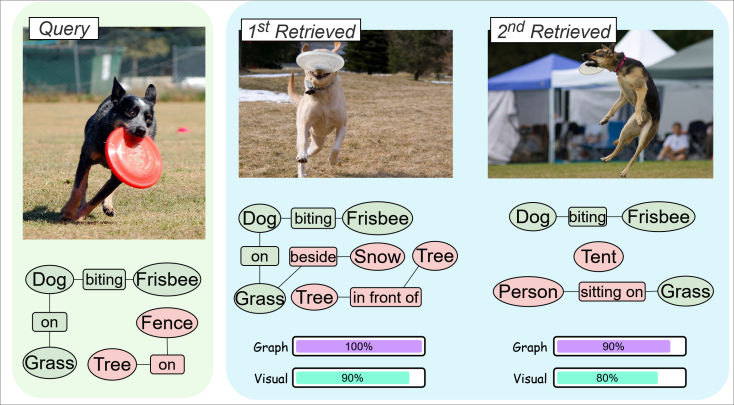
\includegraphics[width=0.7\textwidth]{img/general/acm_prism.png}
        \caption{Top-2 image-to-image visual features, pruning graphs to retain 
            the most important objects and relations, and then encodes objects
            interactions, emphasizing relational structure.} 
    \end{figure}
\end{frame}

\subsection{Methodology}
\begin{frame}{Methodology}
    \begin{block}{Importance Prediction Module}
        Aims to predict \textbf{semantic importance} of both objects and relational triplets \texttt{<subject, relation, object>} through 
        visual and textual cues. It also used \texttt{Human-generated captions} during training as a proxy for semantic relevance.
    \end{block}

    \begin{block}{Edge-Aware Graph Neural Network}
        \begin{itemize}
            \item Refine representation through \texttt{GNN} that integrates both semantic and visual information, 
            which fuses multiple modalities into a \textbf{unified image representation}.
            \item Extend standard attention-based GNNs by encoding edge information during message passing.
        \end{itemize}

        And it is realized in \texttt{Edge-aware Graph Reasoning Module}, which featured in the dual stream. One stream focuses on \textit{Goal Visual Feature}, 
        and other forms \textit{Relational Reasoning}. 
    \end{block}
\end{frame} 

\begin{frame}{Ideas from this paper}
    \begin{block}{Future works}
        This paper introduced a \texttt{image-to-image} retrieval while current direction of team is \texttt{text-to-image} retrieval.

        \begin{itemize}
            \item The \textbf{edges} should encode \texttt{temporal relations} between objects across frames in a video.
            \item Add a \textbf{text encoder stream} on the query side then pair it with a \textbf{visual + graph stream}.
        \end{itemize}
    \end{block}
\end{frame}